\chapter{Bridging the Gap between the Semantic Desktop and the Web of Data}
\label{ch:sdwod}

\begin{flushright}
 \textit{Based on ``Linking Semantic Desktop Data to the Web of Data'' \cite{Dragan2011b}\\published at the 10th International Semantic Web Conference (ISWC~2011)}
\end{flushright}

The previous chapters showed how the Semantic Desktop enables better personal information management on our computers, using semantic technologies to explicitly connect information which is naturally connected in the real-world, and thus matching the representation to a user's mental model. However, our personal data is often a reflection of our subjective view, or limited knowledge. Thus, although it may seem huge when faced with the task of organising it, the information on the desktop is small compared to the amount of information available online. The Web of Data contains a linked network of information similar to the one on the desktop, only at a much larger scale. Connecting the desktop to the Web of Data would enrich and complement desktop information.

This chapter presents a solution to the second research question \textbf{Q 2.} from Section \ref{sub:question}, \emph{how to expand the scope of the Semantic Desktop into the realm of the Web of Data, to enhance the user experience and benefit?}, more specifically, to the first sub-question \textbf{Q 2.1.} described there --- \emph{how to find instances representing the same real-world thing described by a Semantic Desktop resource?}

Our solution uses a semantic search engine for the Web of Data, such as Sindice\footnote{\url{http://sindice.com/}}, to find and retrieve a relevant subset of entities from the Web. We present a matching framework, using a combination of configurable heuristics and rules to compare data graphs, that achieves a high degree of precision for the linking decision.
We evaluate our methodology with real-world data --- we create a gold standard from relevance judgements by experts; and measure the performance of our system against it. We thus show that it is possible to automatically link desktop data with Web data in an effective way.

\section{Introduction}
\label{sec:sdwodintro}

The Semantic Desktop aims to enable better organisation of the personal information on our computers, by applying semantic technologies on the desktop. Just as Linked Data connects distributed data on the Web, creating a network of interlinked information, the Semantic Desktop connects personal data across application boundaries on the desktop, creating a network of personal information.
However, information on our desktop is often incomplete, as it is based on our subjective view, or limited knowledge about an entity.

On the other hand, the Web of Data contains information about virtually everything, generated by multiple sources, and theoretically unlimited. Connecting the desktop to the Web of Data would thus enrich and complement desktop information. Bringing in information automatically from the Web of Data would release the user from the burden of searching for information.

Connecting the two networks of information opens up the possibility of personal services on the desktop, which use external data but in the personal context of the user, highly connected to his personal data and focused on his interests. One such example is a service that finds implicit links between the publications that the user has on the desktop, and provides recommendations to other publications on the same topics, by the same authors, or related in another way. 
Another desktop service could use information from the Web of Data to notify the user of new concert dates in his area, based on the latest or most popular artists played on the desktop. 
Web data can also be used as a point of reference when working collaboratively, e.g., documents linked by the user to people, projects, or other resources from his semantic desktop can be shared together with the annotations, which can be accessed and reused outside of the Semantic Desktop where they were generated.

From the perspective of interlinking information, and using the frameworks provided by the Semantic Desktop and the Web of Data, we have separate islands of knowledge, both containing similar data, related to the same topics of interest to the user, but disconnected from each other. 

The disconnection appears in two forms:
\begin{itemize}
 \item The data on the desktop, although similar to that on the Web of Data, is described using specific \emph{desktop ontologies}, which are different from the ones found on the Web of Data. This schema mismatch makes interlinking data from the two datasets difficult.
 \item Identifiers (URIs) on the desktop are local to the desktop data space, they are not globally unique and cannot be dereferenced as normal Linked Data URIs are. Hence, it is hard to access and connect to local data from the Web.
\end{itemize}

To tackle this disconnection, it is necessary to create links between desktop identifiers and Web identifiers that refer to the same real-world thing.
This means we need to compare the data graph describing an entity on the desktop with the data graph of an entity on the Web. Leaving aside the use of different terminology within the data, the Web of Data is large, with billions of entities across hundreds of thousands of datasets. From this vast amount of information we must find and retrieve a relevant subset of entities, that are potential candidates with the desktop entity. Then we must decide if the candidates are similar enough with the desktop entity to create a link between the two. Because we wish to make the interlinking automatic, we must be able to decide with a high degree of precision which candidates among this subset are in fact referring to the same entity.

Our solution tackles the problems raised above by using a semantic search engine for the Web of Data, such as Sindice, to find and retrieve
a relevant subset of entities from the Web. We then present a matching framework, using a combination of configurable heuristics and rules to
compare data graphs, that achieves a high degree of precision in the linking decision. 

To evaluate our methodology with real-world data, we create a gold standard from relevance judgements by experts, and we measure the performance of our system against it.

Our solution proves that interlinking the two environments is feasible, and even more, it yields good results. Connecting desktop data with the Web enables the system to bring Web data to the users, instead of the users having to go find it by themselves.


\section{Related Work}
\label{sub:sdwodrelatedwork}

The problem of entity linking is well known across various research communities with a variety of different names, such as record linkage \cite{Felligi1969}, entity resolution \cite{Benjelloun2006}, reference reconciliation \cite{Dong2005b} or object consolidation \cite{Hogan2007}. A wide variety of algorithms has been developed for resolving the co-reference problem, but record linkage between distributed databases is still considered a  difficult problem.

Recent initiatives within the Semantic Web community address the problem of linking entities across data sources. For instance, \cite{Jaffri2007} describe the phenomenon of proliferation of URIs and propose a Consistent Reference Service to manage URI equivalences. The OKKAM project \cite{Bouquet2007} proposes an infrastructure for assigning global identifiers at web scale. These approaches are more focussed towards the management of entity identity on the Web, but do not provide an easy means to create new links between data sources. 

Similar to our approach, \cite{Raimond2008} describe an algorithm and its implementation GNAT, for linking a personal music collection to corresponding MusicBrainz resources. The approach recursively measures the similarity of the resource graphs from the two datasets, with the limitation that the same vocabularies must be used in both. By contrast, using property paths in our mappings, we eliminate the need for recursion while still propagating the measures from connected resources.
Silk is a framework for linking multiple entities between two datasets \cite{Bizer2009}. It relies on user-defined rules and various string matching algorithms to measure the similarity between two entities. In this case it is necessary to know a priori which specific dataset to link to and to perform manual configuration of the matching algorithms, something that requires a high degree of expertise.
\cite{Hogan2007} and \cite{Sais2007} propose logic-based methodologies for merging identifiers of equivalent entities across multiples knowledge sources. While being precise, these techniques do not have a very good recall and are computationally demanding.

The most relevant approach related to ours is the Silk framework. We provide a generic matching process that the user can configure based on their own expertise in order to get more precise results. However, our approach differs by the fact that the matching process is not restricted to linking data between two predefined information sources. On the contrary, our approach makes it possible to link desktop data with an arbitrary number of external data sources. This makes the problem harder since we are generally unaware of the data structure or schema of these data sources. 

We therefore need to first find potential entities of interest among a vast number of data sources, then retrieve a partial description of these entities and rely on more complex entity matching algorithms. 

This first step of our algorithm can be seen as a blocking pass to reduce the information space before executing complex matching algorithms \cite{Elmagarmid2007}. The blocking step is implemented on top of a boolean query model for centralised search systems such as Sindice \cite{Tummarello2007} and on top of the SPARQL query language for specific data sources providing a SPARQL endpoint.

\cite{Nikolov2012} propose the use of a genetic algorithm to achieve unsupervised discovery of the similarity parameters needed for data linking between two datasets. Similarly to our algorithm, the approach proposed uses a blocking pass using a SPARQL query, to reduce the computation time. As with Silk, the algorithm considers only two datasets to be matched.


\section{The Process of Finding Web Aliases}
\label{sec:process}

The goal of our algorithm and system is to find Web aliases for desktop resources. A Web alias is a Web entity identifier, i.e., URI, that represents the same real-world thing as the desktop entity to which it was matched. To find Web aliases, we use the information available on the desktop, like the contact information from the address book for people, or metadata of music files for songs, albums and artists. We also use the knowledge about the desktop ontologies and the way data is organised and used on the desktop. The desktop data drives the entire process, and is used throughout the steps:

\begin{enumerate}
 \item Candidate selection --- blocking pass
 \begin{itemize}
  \item Query and identify candidate entities from various Web of Data sources
  \item Retrieve data for each candidate from the appropriate source[s].
 \end{itemize}
 \item Candidate filtering --- scoring based on similarity
 \begin{itemize}
  \item Compute similarity score based on the data of the entities.
  \item Filter the candidates based on the similarity score.
 \end{itemize}
\end{enumerate}

The first step requires identifying a list of candidate entities and obtaining the data available about them. There are two options for this:

\begin{itemize} 
\item through a small set of sources that we know have the data we need, and can query each of them independently for possible candidates, or 
\item through a search engine for the Web of Data, like Sindice \cite{Tummarello2007} which indexes millions of documents containing semantic mark-up.
\end{itemize}
Each option has use cases where it is more suitable than the other, thus we designed our system to support both. Querying specific sources is preferred for instance, if the data is from a very specific domain, like cancer research, or when we are interested only in results from an organisation's internal repository. Using a search engine is best when the information sources to query are not known a priori. It also has the advantage of covering a large number of information sources with only one query, and of selecting the most relevant data sources and candidates with respect to the query via the search engine ranking system. However, in the case of ambiguous entities, the latter option has the disadvantage of returning too many unrelated results, thus making the entity selection more difficult.

Once a list of candidates is available, we compute a similarity score for each of them with respect to the desktop entity. The desktop data is considered authoritative, and the matching process is driven by it. This has the apparent advantage of control, since the desktop data is more strictly under the control of the user. However, there are cases when the desktop data is simply insufficient, or has uncaught errors due to the user's incomplete information, or the Semantic Desktop's extraction process.

The matching algorithm checks first whether the types of the candidate entities correspond to the type of the desktop entity, and discards the ones that do not.
Only then are the data of the entities examined and the properties and corresponding values compared. If required, the algorithm looks at other related entities and their properties. The values of the properties are compared using either exact string matching or string similarity techniques. As mentioned above, the ontologies used on the desktop are different from those used on the Web, thus both type checking and property matching require mappings between the two sets of vocabularies.

After the matching algorithm computes the scores for each of the candidates, the list is filtered for values above a given threshold. References to those Web resources which passed are saved in the desktop repository, as \verb|pimo:hasOtherRepresentation| links from the initial desktop resource.


\section{Implementing the Process}

We implemented the process described above in a desktop daemon that finds Web aliases for desktop entities.
It sequentially searches for aliases for all resources that have no alias listed, and for resources that have changed since the last time aliases were determined for them. In the case when a resource is revisited after being modified, the previously found aliases are discarded and new ones are searched for.

The result of the process is the creation of new links on the Semantic Desktop between local resources and their Web aliases. They can be used to enhance the desktop data about the entities, or as entry points to access further information online.

The implementation has two major components, each handling one step of the matching process: A query component that initiates the search and identifies the candidates, and a matching component that filters the candidates based on similarity measures. We next discuss these components in turn.

\subsection{The Query Component}
\label{sub:querymodule}

The query component was designed to be able to use either generic search engines or specific data sources. Therefore, we chose to make the query module plugin-based, thus allowing various new sources to be connected if needed. The query modules are responsible for finding the initial list of candidates, as well as for retrieving the data for each candidate. The maximum number of candidates to retrieve from a data source can be set as a parameter in the configuration. We allow three types of plugins:
\begin{description}
 \item[SWSE] --- connect to semantic search engines, through their APIs. We provide a plugin of this type for Sindice.
 \item[Sparql] --- connect to sources that provide a SPARQL endpoint. We provide plugins of this type for DBpedia and the Semantic Web Conference Server.
 \item[Custom] --- connect to other sources, possibly ones that do not expose any data as RDF (e.g., relational databases or third-party APIs like last.fm).
 \end{description}

Most major Linked Data providers (e.g. DBpedia) are indexed by Sindice, therefore the Sindice plugin is the only one enabled by default.

In the Sindice module, the initial query, which determines the list of candidates, is constructed using all the value properties of the desktop entity, combined using the boolean conjunction operator ``OR''. Multiple word terms are also tokenised and the tokens are added to the query. This may result into a longer query which contains duplicate words. This is however due to the fact that we rely on the search engine to interpret the query and rank higher the results that match most of the terms. The search engine (in this case Sindice) algorithm ranks higher results which match more of the strings connected by ``OR''. Building the query with just the strings without quotes would result in automatic tokenisation by the search engine, which might lead to higher ranking of unsuitable results, especially if the words searched for are common. Thus we chose to prevent the tokenisation by the search engine by using quotes around the full string searched for, but still mimic the default behaviour of the algorithm by 
doing the tokenisation ourselves, as a fail-safe in case the query yields no results. 

For the music album ``One Night Only'' by the Bee Gees from 1998,  the query constructed is:

\begin{quote}
 \emph{``Bee Gees'' OR ``One Night Only'' OR ``1998'' OR ``Bee'' OR ``Gees'' OR ``One'' OR ``Night'' OR ``Only''}
\end{quote}

\subsection{The Matching Component}
\label{sub:matchingcomp}

The matching module computes a similarity score for each pair $($\emph{desktop~entity}---\emph{web~candidate~entity}$)$. The way the score is computed depends on a set of parameters:

\begin{description}
 \item[String matching (SM)] --- If this parameter is set to \texttt{true}, the matching module will use string similarity measures where appropriate. Currently the system supports Monge-Elkan \cite{Monge1996} and Chapman\footnote{\url{http://sourceforge.net/projects/simmetrics/}} distances. If the value is set to \texttt{false}, the matching module uses exact matching of property values.
 \item[Weighted properties (WP)] --- If \texttt{true}, the matching module will use weights for the properties compared, otherwise, all properties contribute equally to the final score.
 \item[Multi-valued properties (MVP)] --- If \texttt{true}, properties that have more than one matching value will contribute to the score proportionally to the number of values. 
 \end{description}

These parameters are set by default to true. However, the measurements we did for the evaluation (see Section \ref{sec:sdwodeval}) show that in some cases they can be disabled without impacting the quality of the result, while requiring less processing; or even make the algorithm perform slightly better when disabled, for some restrictions.

\lstset{
	caption={Type mapping for pimo:Person.}, 
	label=lst:typemapping,
	language=js
}
\setlength\parindent{0in}
\begin{minipage}[htb]{\linewidth}
\begin{lstlisting}
{
   "http://www.semanticdesktop.org/ontologies/2007/11/01/pimo#Person": {
      "mapping":[
         "http://xmlns.com/foaf/0.1/Person",
         "http://xmlns.com/foaf/0.1/Agent",
         "http://dbpedia.org/ontology/Person",
         "http://www.w3.org/2000/10/swap/pim/contact#Person",
         "http://rdf.data-vocabulary.org#Person" 
      ]
   }
}
\end{lstlisting}
\end{minipage}
\setlength\parindent{0.21in}

\lstset{
	caption={Property mapping for nco:fullname of nmm:performer.}, 
	label=lst:propmapping,
	language=js
}
\setlength\parindent{0in}
\begin{minipage}[htb]{\linewidth}
\begin{lstlisting}
{
   "http://www.semantcdesktop.org/ontologies/2009/02/19/nmm#performer##http://www.semanticdesktop.org/ontologies/2007/03/22/nco#fullname": {
      "mapping": [
         "http://dbpedia.org/property/artist",
         "http://dbpedia.org/ontology/artist##http://xmlns.com/foaf/0.1/name",
         "http://xmlns.com/foaf/0.1/maker##http://xmlns.com/foaf/0.1/name"
      ],
      "approx":"true",
      "thresholds": [
         "MongeElkan:0.7",
         "Chapman:0.8"
      ],
      "weight":"0.7" 
   }
}
\end{lstlisting}
\end{minipage}
\setlength\parindent{0.21in}

The algorithm uses a set of mappings from the desktop ontologies to some of the more popular Web vocabularies, like FOAF. There are two kinds: \emph{type mappings} (see Listing~\ref{lst:typemapping} for an example) and \emph{property mappings}, each described in a separate file. The property mapping supports paths of properties. For example,  Listing~\ref{lst:propmapping} shows a path composed of the property \texttt{dbpedia:artist} and \texttt{foaf:name}. The mappings are relatively static configurations of the system. We have created a set of mappings for the most common ontologies, which can be used out of the box by the end users. Power users can edit the mapping files according to their needs. We envision that as more users find the system useful, more mappings will be created and shared.

\subsubsection{The scoring and matching algorithm}

The algorithm for computing the score works as follows. Given a pair of entities to be compared $e_{d}$ and $e_{w}$, it first determines the sets of types $T_{e_{d}}$ and $T_{e_{w}}$ for each entity, and the set of types $Map[T_{e_{d}}]$ to which the elements of $T_{e_{d}}$ are mapped. If no types are matching, i.e., $T_{e_{w}} \cap Map[T_{e_{d}}] = \phi$, it gives a score $score(e_{w}) = 0$, and stops the matching. Otherwise, it continues the process by evaluating the properties.

The evaluation of the properties is driven by the relations and properties of the desktop entity $e_{d}$. For each property $p_{e_{d}}$, the algorithm retrieves the list of values $V(p_{e_{d}}) = \{v\ :\ \{e_{d}\ p_{e_{d}}\ v\}\}$. Based on the list of property mappings $Map[p_{e_{d}}]$, it determines the set of values $V(p_{e_{w}} \cap Map[p_{e_{d}}])$ that the properties from $Map[p_{e_{d}}]$ have in common with $e_{w}$. If there is no value in common, i.e., $V(p_{e_{d}}) = \phi$ or $V(p_{e_{w}} \cap Map[p_{e_{d}}]) = \phi$, the pair is skipped and nothing is added to the score. Otherwise, it continues the process by measuring the similarity between values.

The evaluation of values is performed using string similarity between each pair of values $(v_{d}, v_{w}) \in V(p_{e_{d}}) \times V(p_{e_{w}} \cap Map[p_{e_{d}}])$. The algorithm creates a sparse matrix where the value of a cell contains a string similarity score between 0 and 1. Let $sum_{p_{e_{d}}}$ be the sum of the best score for each row of the matrix.
The final score is computed as follows:
$$
score(e_{w}) = \frac{\sum_{p_{e_{d}}}(w_{p_{e_{d}}}*sum_{p_{e_{d}}})}{\sum_{p_{e_{d}}}(w_{p_{e_{d}}}*\left|{V(p_{e_{d})}}\right|)}
$$
where $w_{p_{e_{d}}}$ is the weight assigned to a certain property mapping.
If the score is above 0.5\footnote{We found that the threshold 0.5 provided the best results in our experiment.}, the entity is accepted as a Web alias for the desktop entity.
 

\section{Evaluation}
\label{sec:sdwodeval}

To evaluate our system, we wanted to measure the accuracy of the matches, in a real-world set-up, with real data. We only evaluate the matching component of the system, since the query component is straightforward and its performance depends on external factors, like the availability of the services used and the network connection.
To assess the results of the matching, we created two entity corpora, one with desktop data and one with Web data. On these corpora, we first created a baseline from relevance judgements made by human experts. Then, we ran our entity matching algorithm and we computed precision, mean average precision (MAP), and normalised discounted cumulative gain (NDCG) to measure its performance. 

\subsection{Data Collection}

We created two corpora for the evaluation, one containing desktop entities, and one containing possible matching entities from the Web of Data. The Web corpus was obtained by using the query component of the system, with the only active plugin being the Sindice one.

\subsubsection{Desktop data entity corpus}

The desktop data used in the evaluation was collected from a real, in-use Nepomuk-KDE Semantic Desktop. It was generated by Nepomuk applications, and extracted from the desktop repository.

We restricted the entities selected to three types: 
\begin{itemize}
 \item people --- of type \verb|nco:PersonContact|, 
 \item publications --- of type \verb|nfo:PaginatedTextDocument|, and 
 \item music albums --- \verb|nmo:MusicAlbum|.
\end{itemize} 
From each type we collected fifty distinct resources, resulting in a corpus of 150 seed desktop entities, and other entities related to them. Examples of auxiliary entities are the authors of publications, which may or may not be already in the corpus as contacts, the tracks of the albums and the artists. In total the desktop data corpus has 11,917 triples.

We used information from our desktops, therefore the people are colleagues or other researchers we collaborate with; the publications are related to our research interests, and generally related to semantics and information extraction. The music albums data was gathered from several colleagues, for variety of genres.

The contact data is extracted by Nepomuk from the default KDE address book application, and we made no changes to it. The correct way to use the \verb|nco:PersonContact| resources extracted automatically, is to link each of them to a corresponding \verb|pimo:Person| representing the person who has the contact information. However, the current tools do not make the distinction, therefore we also used the ``raw'' \verb|nco:PersonContact| resources, for simplicity. The algorithm makes no distinction between types, so it would yield identical results if we had used the ``proper'' \verb|pimo:Person|.  

The information related to music albums is extracted automatically by Nepomuk from the ID3 tags of music files. 

For publications we used Sclippy\footnote{\url{http://smile.deri.ie/projects/sclippy}}, an existing tool described in \cite{Groza2009}, to perform shallow metadata extraction from files to obtain the title and the authors of the publications, when the metadata of the documents was not set.

\subsubsection{Web of Data entity corpus}

We used the query module of our system to generate the second corpus, containing Web of Data entities. More precisely, we used the Sindice plugin to retrieve the first twenty results returned by Sindice, for each desktop entity, thus making a total of 3,000 URIs. The queries used in Sindice were constructed as presented in Section~\ref{sub:querymodule}, a combination based on the properties of each desktop entity. For each URI we obtained all the triples extracted by Sindice --- explicit and implicit. In total this corpus has 1,530,686 triples.

In this dataset we did not explicitly retrieve Sindice data for the auxiliary entities related to the result URIs. We assumed that this data will be available when and if required --- in the relevance judgements by experts, and in the matching process by the algorithm.

\subsection{Relevance Judgements from Experts}

We collected the relevance judgements from experts through an online experiment, in which we asked participants to decide if pairs of desktop and Web URIs identify the same real-world object or person. We evaluated in this way all 3,000 pairs from the two corpora. Each pair was judged by three different experts. Eighteen people participated in the experiment, all researchers in the area of Semantic Web. 

To simplify the task, we presented the two entities side by side, with all the information which was available about them in the corpora (see Figure~\ref{fig:onlineexperiment}). The desktop entity is shown on the left, and the Web entity on the right. On the Web side we included hyperlinks to the related entities, for further exploration in case the information given was not sufficient for making the decision. For convenience, on the Web side, we have separated and brought to the top the triples which partially matched any of the values from the desktop side. 

\begin{figure}[htb]
 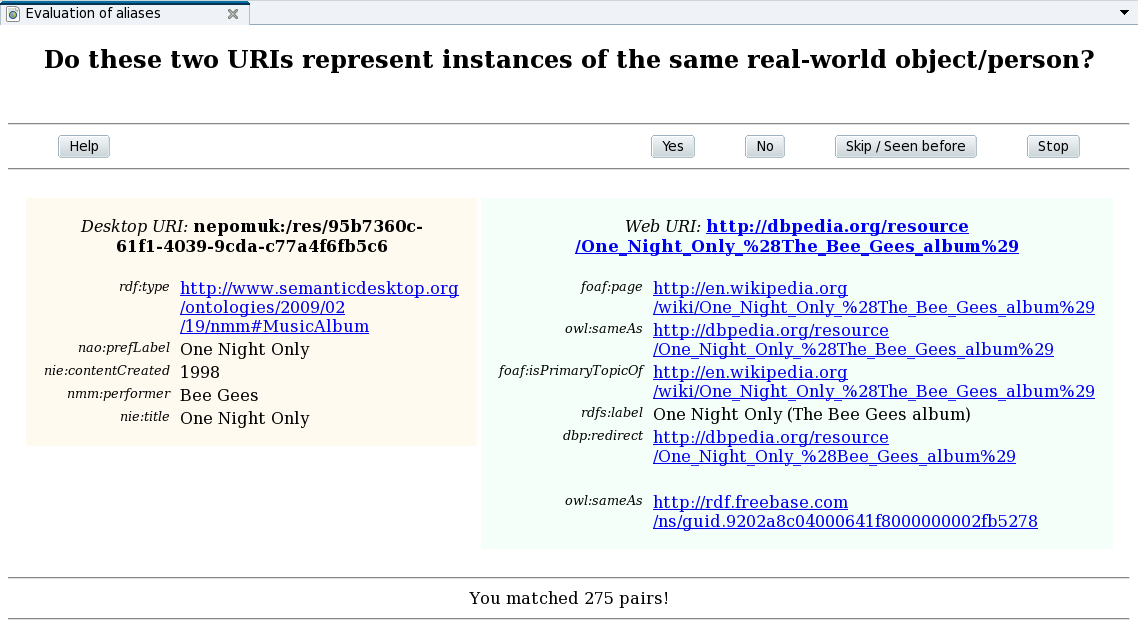
\includegraphics[width=\linewidth]{chapters/core/img/eval_album.png}
\caption{The Web interface of the experiment for collecting relevance judgements.}
\label{fig:onlineexperiment}
\end{figure} 

There were only two decisions possible: \emph{Yes} or \emph{No}, with a \emph{Skip} option, in case of uncertainty. Once a pair was judged or skipped, another one was shown to the participant. The pairs were randomly chosen from the remaining set. To add a gamification element to the experiment, we kept count of the number of pairs judged by each participant, and displayed it on the page. We found that even such a small addition generated ad-hoc competition and made the dull task more interesting.

The results of the experiment show an average agreement and its standard deviation, computed with Fleiss's $\kappa$, of $0.638\pm0.214$, over all three types of entities, suggesting substantial agreement between annotators. Table~\ref{tab:agreementsdwod} shows the Fleiss's $\kappa$ and its standard deviation $\sigma$ per type, as well as the average pairwise percent agreement. We observed that for music albums, there was only moderate agreement between annotators, visibly lower than the average, while for publications it is visibly higher. We believe the difference is caused by the fact that the data about publications is generated and curated by experts in the field --- even more so, as the publications were largely from the domain of Semantic Web --- while the music data comes from much more heterogeneous sources.

\begin{table}
\centering
\ra{1.3}
\begin{tabular}{@{}rcl@{\hs}l@{\hs}l@{}}
\toprule
& \phantom{a} & $\kappa$ & $\sigma$ & Avg  \\ 
\midrule

 All && 0.638 & 0.214 & 92.252 \\

 People && 0.661 & 0.257 & 88.2 \\

 Publications && 0.786 & 0.127 & 98.067  \\

 Albums && 0.442 & 0.233 & 90.523 \\

\bottomrule
\end{tabular}
\caption{Inter-annotator agreement measures}
\label{tab:agreementsdwod}
\end{table}

\subsection{Quantitative Results}

To evaluate the performance of the algorithm, we evaluate each of the matching parameters described in Section \ref{sub:matchingcomp}, activated either separately or using a combination of them, against a baseline which is the matching framework with all the parameters disabled. In the following, the String Matching parameter is denoted by SM, the Weighted Properties by WP and the Multi-Valued Properties by MVP.

We used the \emph{trec\_eval} tool\footnote{\url{http://trec.nist.gov/trec_eval/}} to compute standard information retrieval measures.
The precision at k ($P@k$) with k={1,2,3,4,5}, mean average precision (MAP) and normalised discounted cumulative gain (NDCG) are reported in Table~\ref{tab:agreement-albums} for music albums, Table~\ref{tab:agreement-people} for people and Table~\ref{tab:agreement-publications} for publications. 
We report also the interpolated precision at recall cut-off points when all matching parameters are enabled. The goal for the system is high precision, i.e., achieving a maximum at P@1. Recall is not a target, as it is generally impossible to determine the entire set of correct results available in the Web of Data.

\begin{table}[htb]
\centering
\ra{1.3}
\begin{tabular}{@{}rcl@{\hs}l@{\hs}l@{\hs}l@{\hs}l@{\hs}l@{\hs}l@{}}
\toprule
& \phantom{a} & MAP & NDCG & P@1 & P@2 & P@3 & P@4 & P@5 \\ 
\midrule

 SM WP MVP && 0.2464 & 0.5117 & 1 & 0.625 & 0.4167 & 0.3125 & 0.25 \\ %111

 SM WP && 0.2464 & 0.5117 & 1 & 0.625 & 0.4167 & 0.3125 & 0.25 \\ %110

 SM MVP && 0.2464 & 0.5117 & 1 & 0.625 & 0.4167 & 0.3125 & 0.25 \\ %101

 WP MVP && 0 & 0 & 0 & 0 & 0 & 0 & 0 \\ %011

 SM && 0.2464 & 0.5117 & 1 & 0.625 & 0.4167 & 0.3125 & 0.25 \\ %100

 WP && 0 & 0 & 0 & 0 & 0 & 0 & 0 \\ %010

 MVP && 0 & 0 & 0 & 0 & 0 & 0 & 0 \\ %001

 Baseline && 0 & 0 & 0 & 0 & 0 & 0 & 0 \\ %000

\bottomrule
\end{tabular}
\caption{Evaluation results for albums, when varying configuration parameters.}
\label{tab:agreement-albums}
\end{table}

In Table~\ref{tab:agreement-albums}, we can observe that only the SM parameter is enhancing the results compared to the baseline. The other two parameters do not improve the results at matching certain candidates. Also, in term of MAP and NDCG, the system achieves the lowest performance on the albums corpus. This can be explained by the fact that the Web resources returned by the query module for albums are mostly e-commerce products, which are not defined as a type of interest, and therefore are rejected by the matching module. However, some of the annotators have considered that the corresponding candidates are indeed the same as the album, while some have disagreed --- this is reflected in the agreement measure, as for the albums we have the lowest value for Fleiss's $\kappa$. Whether or not such candidates should have been kept by the system is open to discussion and left for future work.

\begin{table}[htb]
\centering
\ra{1.3}
\begin{tabular}{@{}rcl@{\hs}l@{\hs}l@{\hs}l@{\hs}l@{\hs}l@{\hs}l@{}}
\toprule
& \phantom{a} & MAP & NDCG & P@1 & P@2 & P@3 & P@4 & P@5 \\ 
\midrule

 SM WP MVP && 0.4212 & 0.6354 & 0.9302 & 0.8953 & 0.7597 & 0.6337 & 0.5442 \\ %111

 SM WP && 0.4174 & 0.6321 & 0.9286 & 0.8929 & 0.746 & 0.6131 & 0.5286 \\ %110

 SM MVP && 0.4212 & 0.6354 & 0.9302 & 0.8953 & 0.7597 & 0.6337 & 0.5442 \\ %101

 WP MVP && 0.2916 & 0.5338 & 1 & 0.8243 & 0.6036 & 0.473 & 0.3838 \\ %011

 SM && 0.4212 & 0.6354 & 0.9302 & 0.8953 & 0.7597 & 0.6337 & 0.5442 \\ %100

 WP && 0.2916 & 0.5338 & 1 & 0.8243 & 0.6036 & 0.473 & 0.3838 \\ %010

 MVP && 0.2877 & 0.53 & 1 & 0.8243 & 0.6036 & 0.4662 & 0.3784 \\ %001

 Baseline && 0.2877 & 0.53 & 1 & 0.8243 & 0.6036 & 0.4662 & 0.3784 \\ %000

\bottomrule
\end{tabular}
\caption{Evaluation results for people, when varying configuration parameters.}
\label{tab:agreement-people}
\end{table}

In Table~\ref{tab:agreement-people}, we can observe that the baseline, the WP and the MVP parameters are each able to match good candidates with high precision at P@1, with WP providing slightly better MAP and NDCG. However, the system does not get significant advantage by combining them. The SM parameter alone provides slightly lower precision at P@1 but significantly better MAP and NDCG. By combining the three parameters, the system does not get significant advantage and it seems that using SM prevails. 

\begin{table}[htb]
\centering
\ra{1.3}
\begin{tabular}{@{}rcl@{\hs}l@{\hs}l@{\hs}l@{\hs}l@{\hs}l@{\hs}l@{}}
\toprule
& \phantom{a} & MAP & NDCG & P@1 & P@2 & P@3 & P@4 & P@5 \\ 
\midrule

 SM WP MVP && 0.7773 & 0.8651 & 1 & 0.625 & 0.4167 & 0.3125 & 0.25 \\ %111

 SM WP && 0.8032 & 0.8609 & 0.9062 & 0.5781 & 0.3958 & 0.3047 & 0.2438 \\ %110

 SM MVP && 0.7175 & 0.7986 & 0.9231 & 0.5769 & 0.3846 & 0.2885 & 0.2308 \\ %101

 WP MVP && 1 & 1 & 1 & 0.5 & 0.3333 & 0.25 & 0.2 \\ %011

 SM && 0.7265 & 0.7883 & 0.8235 & 0.5294 & 0.3627 & 0.2868 & 0.2294 \\ %100

 WP && 0.6893 & 0.7347 & 1 & 0.55 & 0.3667 & 0.275 & 0.22 \\ %010

 MVP && 0 & 0 & 0 & 0 & 0 & 0 & 0 \\ %001

 Baseline && 0.7175 & 0.7588 & 1 & 0.5455 & 0.3636 & 0.2727 & 0.2182 \\ %000

\bottomrule
\end{tabular}
\caption{Evaluation results for publications, when varying configuration parameters.}
\label{tab:agreement-publications}
\end{table}

In Table~\ref{tab:agreement-publications}, the baseline provides good results from the start for publications. The system is not able to return any candidates when MVP alone is activated. However, when WP and MVP are combined, the system achieves much better results (in term of MAP and NDCG) than the baseline or than the WP parameter alone. When the system combines SM with the two previous ones, the system achieves a lower MAP and NDCG but an improved precision with a larger cut-off rank. While on the two previous types of entities, the SM parameter seemed to be the most important matching feature, this corpus shows that the WP and MVP are important matching features in certain cases.

\begin{figure}[htb]
 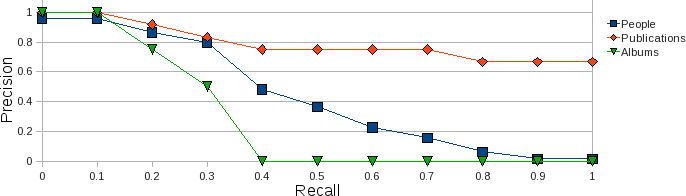
\includegraphics[width=\linewidth]{chapters/core/img/precrecal_wlabels.png}
\caption{Interpolated precision at recall cut-off points.}
\label{fig:precrecall}
\end{figure}

Overall, the results are satisfying for our use cases where high precision prevails over recall. However, given the results shown in Figure~\ref{fig:precrecall}, we can see that the system could be configured to return more than one entity in order to achieve better recall while keeping good precision. It might prove useful to implement a semi-automatic system which presents the top \emph{n} candidates to the user for manual selection.

\subsection{Performance}

To determine the performance, we measured the time spent on each step of the algorithm. We note that these results come from a prototype implementation, still to be subject to technical optimisations. Table~\ref{tab:sdwodtimes} shows the average times overall, and for each resource type separately, when all three parameters (SM, WP, MVP) are active. We find only small variations in the measurements when the parameter values are changed. We do not consider the time spent on retrieving data from Sindice, as this depends on external factors, like network speed and server availability. 

\begin{table}[htb]
\centering
\ra{1.3}
\begin{tabular}{@{}rcr@{\hs}r@{\hs}r@{\hs}r@{}}
\toprule
& \phantom{a} & Overall & People & Publications & Albums \\ 
\midrule

 Pair total && 375.04 & 52.19 & 977.87 & 53.18 \\

 Types check && 0.23 & 0.26 & 0.21 & 0.23 \\

 Per property check && 6.66 & 0.92 & 13.2 & 22.06 \\

 All properties && 2026.22 & 7.17 & 5478.87 & 1963.88 \\

\bottomrule
\end{tabular}
\caption{Time performance (milliseconds).}
\label{tab:sdwodtimes}
\end{table}

The checking of types is the only value that on average does not depend on the type of resource, as it must be performed for all pairs. The time spent in average per property check is low, but it varies by type, and by the complexity of the properties (e.g. it takes longer if several resources in the graph must be traversed, for long property paths like the name of the artist of an album). The ``All properties'' row shows the average time required for checking all the properties of an entity, and the computation of the final score\footnote{The ``All properties'' row has values higher that the ``Pair total'' row because the average time is computed only for those pairs that passed the type check, thus fewer, but with longer computation times.}. These values depend on the type of resources as well, and on the complexity of the resource graph. We found that longer times correspond to very big graphs for online entities, which must be loaded for checking even if in most cases are not found to represent valid 
candidates\footnote{e.g., the graph for \url{http://webconf.rkbexplorer.com/models/iswc-aswc-2007-complete.
rdf}}.


\section{Discussion}

The scope of the system presented here is limited to finding Web of Data aliases for desktop resources. We leave the use of the aliases found to future work, but the use cases include personalised desktop services like those described in Section~\ref{sec:sdwodintro} and enhancement of desktop information from online sources like the one described in \cite{Groza2009}. We plan to develop a semi-automatic service that retrieves information from the Web aliases and updates the local resources, while saving provenance information for the imported data and allowing synchronisation when the Web data changes.

Existing Web applications already provide similar services via specific APIs (e.g., last.fm). However this is not the goal of our work. Instead, we wish to leverage information across all public information sources accessible on the Web of Data. In addition, such third-party APIs are seen as an additional information sources on the Web, and are supported by our system.

Within the system, we make use of existing semantic technologies, including semantic search engines such as Sindice. In the process of determining the aliases we focus on selecting the most appropriate URI from the list of candidates returned by the search engine. In this case, the issue of which data sources to trust is left to the search engine, which usually employs advanced techniques~\cite{Delbru2010} for making the decision. This is however not a requirement we impose on the users, who can choose to query other trusted data sources suitable for their use case.

The system we presented is automatic, as no user interaction is required for it to work. Once set up it will find and save aliases to desktop resources. 
Although the mappings were created manually, they are part of the system and do not need to be modified by end users. 
Power users can however tweak the settings to fit their specific needs by enabling or disabling modules, changing threshold values or modifying mappings.
While new mappings can only be created manually, expert users can take advantage of the openness resulting from the use of SPARQL-based search mechanism and update the mappings as they need, or create new ones. We envision for the future, a way of allowing power users to publish their own mappings and let other users install new mappings in a way similar to installing add-ons to Web browsers.


\section{Conclusion}

In this chapter, we presented a framework to automatically link entities from the Semantic Desktop to the Web of Data. This is the logical next step after the creation of semantic data on the desktop, presented in the previous chapter.

The framework uses existing technologies such as semantic search engines and public SPARQL endpoints for retrieving a set of candidates. Each candidate is then evaluated more precisely based on a collection of matching components using string matching, heuristics and rule-based mechanisms. We evaluate the system qualitatively, using real-world data retrieved from a Nepomuk-KDE Semantic Desktop and the Sindice search engine. The evaluation is based on relevance judgements from a group of experts. We show that the system in its current form provides satisfactory results in term of precision for automatic linking of entities.

Once the two networks of linked data are connected, we can build semantic applications and services using personal data from the desktop and enriched with information from the Web of Data. In the next chapter we present one such application.
